\documentclass[12pt,a4paper]{report}
\usepackage[utf8]{inputenc}
\usepackage[left=1.25in,right=1in,top=1in,bottom=1in]{geometry}
\usepackage{amsmath,amssymb}
\usepackage{graphicx}
\usepackage{booktabs,array}
\usepackage{tikz}
\usetikzlibrary{arrows.meta,positioning,shapes.geometric,calc}
\usepackage[hidelinks]{hyperref}

\linespread{1.3}

\newcommand{\cmode}{C-MODE}
\newcommand{\JSD}{\operatorname{JSD}}
\newcommand{\ind}{\mathbf{1}}

\tikzset{
  box/.style={draw,rounded corners=2pt,align=center,font=\footnotesize,minimum height=7mm,text width=38mm,inner sep=4pt},
  decision/.style={draw,diamond,aspect=2.2,align=center,font=\scriptsize,inner sep=1pt,text width=24mm},
  arr/.style={-{Latex[length=1.5mm]},thick}
}

\begin{document}

% ==============================================================================
% 1. TITLE PAGE
% ==============================================================================
\begin{titlepage}
\begin{center}
\vspace*{0.2cm}
{\Large \bfseries GENRAGA: AN EVOLUTIONARY ARTIFICIAL INTELLIGENCE FRAMEWORK FOR CARNATIC MUSIC GENERATION WITH CONSTRAINED MULTI-OBJECTIVE OPTIMIZATION AND EMPIRICAL GAMAKA SYNTHESIS \par}
\vspace{1.5cm}
{\large \bfseries 24CS798 -- DISSERTATION PHASE -- I \par}
\vspace{1.2cm}
{\large Submitted by \par}
\vspace{0.4cm}
{\large \bfseries SHRINIDHI MAHESHWARAN [CB.SC.P2CSE25033] \par}
\vspace{1.2cm}
{\large in partial fulfillment of the requirements for the degree of \par}
\vspace{0.4cm}
{\large \bfseries MASTER OF TECHNOLOGY \par}
{\large \bfseries in \par}
{\large \bfseries COMPUTER SCIENCE AND ENGINEERING \par}
\vspace{1.8cm}
{\bfseries DEPARTMENT OF COMPUTER SCIENCE AND ENGINEERING \par}
{\bfseries AMRITA SCHOOL OF COMPUTING \par}
{\bfseries AMRITA VISHWA VIDYAPEETHAM \par}
{\bfseries COIMBATORE -- 641 112 \par}
\vspace{1.2cm}
{\large \bfseries NOVEMBER 2026 \par}
\end{center}
\end{titlepage}

% ==============================================================================
% 2. BONAFIDE CERTIFICATE
% ==============================================================================
\newpage
\thispagestyle{empty}
\begin{center}
{\Large \bfseries AMRITA VISHWA VIDYAPEETHAM \par}
{\bfseries AMRITA SCHOOL OF COMPUTING, COIMBATORE \par}
{\bfseries DEPARTMENT OF COMPUTER SCIENCE AND ENGINEERING \par}
\vspace{1.2cm}
{\large \bfseries BONAFIDE CERTIFICATE \par}
\end{center}
\vspace{0.8cm}

This is to certify that the thesis entitled \textbf{``GENRAGA: AN EVOLUTIONARY ARTIFICIAL INTELLIGENCE FRAMEWORK FOR CARNATIC MUSIC GENERATION WITH CONSTRAINED MULTI-OBJECTIVE OPTIMIZATION AND EMPIRICAL GAMAKA SYNTHESIS''}, submitted by \textbf{SHRINIDHI MAHESHWARAN [CB.SC.P2CSE25033]}, in partial fulfillment of the requirements for the award of degree of \textbf{Master of Technology in Computer Science and Engineering}, is a bonafide record of the research work carried out under my guidance and supervision at the Department of Computer Science and Engineering, Amrita School of Computing, Amrita Vishwa Vidyapeetham, Coimbatore.

\vspace{3.5cm}
\noindent
\begin{tabular}{@{}p{0.5\textwidth}p{0.5\textwidth}@{}}
\textbf{Dr. Ritwik M} & \textbf{Dr. P. Bagavathi Sivakumar} \\
Thesis Advisor & Chairperson \\
Department of Computer Science & Department of Computer Science \\
and Engineering & and Engineering \\
Amrita School of Computing & Amrita School of Computing \\
Coimbatore -- 641 112 & Coimbatore -- 641 112 \\
\end{tabular}

\vspace{2.5cm}
\noindent
\textbf{Evaluated on:} \rule{4cm}{0.4pt}

\vspace{1.5cm}
\noindent
\begin{tabular}{@{}p{0.5\textwidth}p{0.5\textwidth}@{}}
\rule{5cm}{0.4pt} & \rule{5cm}{0.4pt} \\
\textbf{Internal Examiner} & \textbf{External Examiner} \\
\end{tabular}

% ==============================================================================
% 3. ACKNOWLEDGEMENT
% ==============================================================================
\newpage
\pagenumbering{roman}
\setcounter{page}{3}
\begin{center}
{\Large \bfseries ACKNOWLEDGEMENT \par}
\end{center}
\vspace{0.8cm}

I would like to express my deep sense of gratitude and devotion to our beloved Chancellor \textbf{Satguru Sri Mata Amritanandamayi Devi} for providing an inspiring academic climate and spiritual environment in this university, which has made the successful completion of this research work possible.

I would like to thank the management of \textbf{Amrita Vishwa Vidyapeetham} and the entire faculty fraternity of the Department of Computer Science and Engineering, Amrita School of Computing, Coimbatore, for providing the necessary computing resources, infrastructure, and technical guidance required for this dissertation.

I wish to record my profound gratitude and sincere thanks to my research supervisor, \textbf{Dr. Ritwik M}, for his invaluable suggestions, technical insights, and continuous encouragement throughout all phases of this project. His deep expertise in evolutionary computation and constructive critique were pivotal in shaping the algorithmic design and empirical validation of GenRaga.

I also extend my heartfelt thanks to \textbf{Dr. P. Bagavathi Sivakumar}, Chairperson, Department of Computer Science and Engineering, and the members of the Dissertation Review Committee for their critical evaluation and valuable recommendations.

Finally, I express my deepest appreciation to my family, friends, and fellow research scholars for their constant moral support, patience, and encouragement throughout my postgraduate studies.

\vspace{1.5cm}
\noindent
\textbf{SHRINIDHI MAHESHWARAN} \\
CB.SC.P2CSE25033

% ==============================================================================
% 4. ABSTRACT
% ==============================================================================
\newpage
\begin{center}
{\Large \bfseries ABSTRACT \par}
\end{center}
\vspace{0.8cm}

Synthesizing authentic Carnatic melodies requires strictly enforcing complex modal grammars, continuous microtonal pitch inflections, and cyclic metric grids. In South Indian classical music, melodic identity is defined by the interaction of modal rules (\textit{raga}), continuous microtonal dynamics (\textit{gamaka}), and cyclic metric frameworks (\textit{tala}). Conventional deep generative neural networks frequently fail in this domain because statistical sampling across discrete MIDI tokens cannot guarantee scale legality, forbidden (\textit{varjya}) intervallic leaps, or cyclic metric cadence.

This thesis presents \textbf{GenRaga}, an interpretable artificial intelligence framework that models Carnatic melody generation as a Constrained Multi-Objective Differential Evolution (\cmode) problem over corpus-derived rhythmic phrase cells. Operating on a consolidated multi-source manifest of 705 recording tracks spanning 103 raga classes, we extract formal grammar transition move graphs across seven primary foundation ragas (\textit{Mohanam}, \textit{Kalyani}, \textit{Abhogi}, \textit{Begada}, \textit{Sahana}, \textit{Saveri}, \textit{Sri}). Compositions are parameterized as discrete sequences of rhythmic akshara cells and optimized through continuous 9-dimensional feature-space differential vector mutations, nearest-neighbor legal snapping, constraint join repairs, and NSGA-II non-dominated sorting over five competing musical proxy objectives. Continuous audio rendering is achieved by coupling generated swara skeletons with empirical microtonal residual contours extracted from 27,731 dynamic-time-warped performance notes across 28 concert vocal recordings.

Under balanced constraint topologies, \cmode\ achieves consistent Pareto hypervolume gains over random-walk baselines across all seven foundation ragas (+30.2\% in Begada, +29.8\% in Sri, +13.2\% in Mohanam, +9.2\% in Sahana, +8.0\% in Saveri, +7.6\% in Abhogi, and +1.4\% in Kalyani) with 100\% structural validity. In strict constraint mode, \cmode\ prevents the premature genetic drift observed in weighted-sum genetic algorithms, outperforming them in 100\% of matched seed runs. Synthesized audio pieces attain a median pitch error of 0.824 cents, with an internal calibrated 42-class raga classifier achieving 94.4\% identification accuracy. Furthermore, a formal double-blind listening field study with $N=30$ Carnatic musicians and listeners demonstrates an overall composite rating of 4.30 / 5.0 and a 74.4\% Turing pass rate. These results establish GenRaga as an effective, inspectable computational framework for automated composition in rule-governed art music traditions.

% ==============================================================================
% 5. TABLE OF CONTENTS, TABLES, FIGURES
% ==============================================================================
\newpage
\tableofcontents

\newpage
\listoftables

\newpage
\listoffigures

% ==============================================================================
% 6. ABBREVIATIONS & SYMBOLS
% ==============================================================================
\newpage
\begin{center}
{\Large \bfseries ABBREVIATIONS \par}
\end{center}
\vspace{0.8cm}

\noindent
\begin{tabular}{@{}ll@{}}
\textbf{AI} & Artificial Intelligence \\
\textbf{CFG} & Context-Free Grammar \\
\textbf{C-MODE} & Constrained Multi-Objective Differential Evolution \\
\textbf{CMD} & CompMusic Carnatic Dataset \\
\textbf{DE} & Differential Evolution \\
\textbf{DTW} & Dynamic Time Warping \\
\textbf{EA} & Evolutionary Algorithm \\
\textbf{FAD} & Fr{\'e}chet Audio Distance \\
\textbf{GA} & Genetic Algorithm \\
\textbf{HV} & Hypervolume Metric \\
\textbf{JSD} & Jensen-Shannon Divergence \\
\textbf{MIR} & Music Information Retrieval \\
\textbf{NSGA-II} & Non-dominated Sorting Genetic Algorithm II \\
\textbf{RRD} & Raga Recognition Dataset \\
\textbf{TPM} & Transition Probability Matrix \\
\textbf{VNS} & Variable Neighborhood Search \\
\end{tabular}

\newpage
\begin{center}
{\Large \bfseries LIST OF SYMBOLS \par}
\end{center}
\vspace{0.8cm}

\noindent
\begin{tabular}{@{}ll@{}}
$S, R, G, M, P, D, N$ & Seven primary solf{\`e}ge swaras (Shadja, Rishabha, Gandhara, etc.) \\
$S_-, S, S^+$ & Lower octave, middle octave, and upper octave swara markers \\
`,` & Swara elongation / sustained hold token \\
$f_0$ & Fundamental frequency of performance tonic in Hertz \\
$c(t)$ & Pitch in continuous cents relative to tonic reference \\
$E(g)$ & 9-dimensional standardized musical feature vector of cell $g$ \\
$\mathcal{J}(u_1, u_2)$ & Boundary junction validity tuple $(s_{\text{last}}, s_{\text{first}}, h_{\text{lead}})$ \\
$\mathcal{L}(g)$ & Set of legally permissible successor cells following cell $g$ \\
$F$ & Differential Evolution mutation scale factor, $F \sim U(0.4, 0.9)$ \\
$CR$ & Differential Evolution binomial crossover probability ($CR = 0.7$) \\
$f_1$ & Raga Melodic Fidelity Objective Function \\
$f_2$ & Gamaka Readiness Objective Function \\
$f_3$ & Tala Metric Alignment Objective Function \\
$f_4$ & Melodic Diversity Objective Function \\
$f_5$ & Section and Register Structure Objective Function \\
$\mathcal{F}_0$ & Non-dominated Pareto frontier set \\
$\delta c(t)$ & Empirical gamaka microtonal residual curve in cents \\
\end{tabular}

% ==============================================================================
% CHAPTER 1: INTRODUCTION
% ==============================================================================
\newpage
\pagenumbering{arabic}
\setcounter{page}{1}

\chapter{Introduction}

\section{Motivation and Problem Statement}
The development of generative artificial intelligence for music has progressed rapidly with deep connectionist models capable of generating high-fidelity audio streams from natural language prompts~\cite{copet2023}. However, standard generative architectures are fundamentally tailored to Western equal-tempered tonal systems characterized by discrete pitches, chord progressions, and fixed-meter time signatures. 

Carnatic music, the classical music tradition of South India, represents a vastly different musical paradigm rooted in explicit modal grammar, continuous microtonal pitch dynamics, and asymmetric cyclic rhythm. These core characteristics form three interdependent structural pillars:
\begin{enumerate}
    \item \textbf{Raga (Melodic Grammar):} A raga is not merely a collection of permissible scale degrees. It defines rigid ascending (\textit{arohana}) and descending (\textit{avarohana}) pitch paths, specifies forbidden (\textit{varjya}) intervals, establishes primary melodic centers (\textit{vadi/samvadi}), and prescribes signature phrase motifs (\textit{prayoga}).
    \item \textbf{Gamaka (Continuous Microtonality):} Ornamentation in Carnatic music is not an acoustic embellishment such as vibrato. Rather, it is an essential structural property of swara identity consisting of microtonal glides, kampita oscillations, and contextual pitch inflections~\cite{gamaka2022}.
    \item \textbf{Tala (Cyclic Metric Framework):} Rhythm is structured as repetitive metric cycles (\textit{avartanams}) partitioned into asymmetric structural pulses (\textit{angas}) and subdivided beat units (\textit{aksharas}), frequently requiring melodies to launch at off-beat offsets (\textit{eduppu}).
\end{enumerate}

Standard deep generative models and discrete MIDI representations fail in this domain. Statistical neural decoders cannot provide formal guarantees that generated melodies will avoid forbidden scale intervals or conform to cyclic tala boundaries. When algorithmic composition requires verifiable structural compliance, black-box statistical generators must be replaced by inspectable, constraint-governed optimization frameworks.

\section{Research Objectives}
To address these challenges, this research pursues the following concrete objectives:
\begin{enumerate}
    \item \textbf{Corpus Ingestion \& Grammar Extraction:} To aggregate a consolidated multi-source manifest of Carnatic audio and pitch records, and extract context-free structural grammars across seven primary foundation ragas.
    \item \textbf{Evolutionary Multi-Objective Algorithm Design:} To develop \cmode, an adaptation of Differential Evolution operating in a continuous 9-dimensional musical feature space with discrete legal snapping and NSGA-II Pareto optimization.
    \item \textbf{Empirical Gamaka Synthesis Pipeline:} To establish an empirical microtonal synthesis bank by aligning 27,731 individual notes from 28 concert vocal performances using Dynamic Time Warping (DTW), eliminating synthetic pitch-bend artifacts.
    \item \textbf{Systematic Benchmark Evaluation:} To benchmark \cmode\ against random-walk and weighted-sum genetic algorithm baselines under equal computational budgets across all seven foundation ragas.
    \item \textbf{Human Perceptual Validation:} To conduct a formal double-blind listening field study with $N=30$ Carnatic musicians and listeners evaluating grammar conformance, gamaka naturalness, and Turing-style discrimination.
\end{enumerate}

\section{Key Contributions}
The main contributions of this thesis are:
\begin{enumerate}
    \item An inspectable, end-to-end framework linking heterogeneous Carnatic corpora, rhythmic cell grammars, multi-objective evolutionary search, and recording-derived gamaka rendering.
    \item The formulation and implementation of \cmode, enabling continuous DE vector mutations over discrete musical phrases via standardized feature embeddings and constraint join repairs.
    \item A comprehensive 7-raga empirical benchmark demonstrating that balanced-mode \cmode\ achieves significant hypervolume gains over random walks (up to +30.2\% in Begada and +29.8\% in Sri) while maintaining 100\% structural validity.
    \item A rigorous theoretical and empirical analysis of why multi-objective Pareto optimization prevents the linear compensation trap and premature genetic drift that plagues weighted-sum genetic algorithms.
    \item A published 8-page IEEE conference paper with 40 references, an interactive live 3-instrument web studio, and an empirical field evaluation report.
\end{enumerate}

\section{Thesis Organization}
The remainder of this thesis is structured as follows:
\begin{itemize}
    \item \textbf{Chapter 2 (Literature Survey):} Reviews evolutionary music composition, Indian classical music information retrieval, microtonal gamaka synthesis, and identifies critical research gaps.
    \item \textbf{Chapter 3 (Proposed System Architecture):} Details the overall GenRaga architecture, dataset curation, hierarchical cell representation, grammar move graphs, and natural-language query routing.
    \item \textbf{Chapter 4 (C-MODE Algorithmic Formulations):} Provides complete mathematical definitions of the 9D feature embedding, differential mutation, legal snapping, five objective functions, NSGA-II selection, and DTW gamaka retrieval.
    \item \textbf{Chapter 5 (Implementation and Experimental Evaluation):} Presents benchmark results across all seven ragas, theoretical C-MODE vs. Weighted GA comparisons, audio pitch accuracy, classification results, and documented failure modes.
    \item \textbf{Chapter 6 (Conclusion and Future Scope):} Summarizes major research findings, practical implications for musicology, system limitations, and outlines directions for future research.
\end{itemize}

% ==============================================================================
% CHAPTER 2: LITERATURE SURVEY
% ==============================================================================
\chapter{Literature Survey}

\section{Evolutionary Algorithms in Music Composition}
Evolutionary computation has a rich history in algorithmic music composition dating back to early rule-based genetic algorithms for species counterpoint and motivic interpolation~\cite{mcintyre1994,horner1991,maddox2000}. In Western classical music, initial systems concentrated on four-part harmonization using penalty functions derived from classical voice-leading rules~\cite{donnelly2011,donnelly2012,phonamnuaisuk1999}. Herremans and S{\"o}rensen~\cite{herremans2012,herremans2013} demonstrated that metaheuristics such as Variable Neighborhood Search (VNS) navigate contrapuntal constraints effectively when decomposed into quantified sub-scores.

In melodic extension and style imitation, Towsey \textit{et al.}~\cite{towsey2001}, Marques \textit{et al.}~\cite{marques2000}, and Mati{\'c}~\cite{matic2010} explored multi-feature fitness functions capturing pitch contour, interval entropy, and rhythmic repetition. Recombinant composition based on corpus statistics was advanced by Eigenfeldt~\cite{eigenfeldt2012} and De Prisco \textit{et al.}~\cite{deprisco2020}, who extracted statistical n-grams from Bach chorales to balance structural rule-following with stylistic fidelity. To model hierarchical musical form, Hofmann~\cite{hofmann2015} deployed Genetic Programming over tree-structured phrases.

Hybrid systems combining evolutionary search with neural evaluators emerged early with Burton and Vladimirova~\cite{burton1998}, and were expanded by Farzaneh and Toroghi~\cite{farzaneh2019,farzaneh2020} using recurrent networks for interactive and generative melody creation. Majidi and Toroghi~\cite{majidi2022} integrated multi-objective genetic algorithms with deep learning fitness evaluators for polyphonic harmony.

In improvisational and jazz domains, Biles' GenJam~\cite{biles1994,biles2001} pioneered real-time interactive genetic algorithms for solo generation, later extended through rule-based and machine-learning fitness functions by Papadopoulos and Wiggins~\cite{papadopoulos1998}, {\"O}zcan and Er{\c{c}}al~\cite{ozcan2008}, and Liu and Ting~\cite{liuting2019}. Macro-structural affective generation was explored by Scirea \textit{et al.}~\cite{scirea2017} with MetaCompose. Beyond fixed-length representations, grammatical evolution and information-theoretic fitness functions based on Zipf's law were developed by Alfonseca \textit{et al.}~\cite{alfonseca2007}, Manaris \textit{et al.}~\cite{manaris2003}, Loughran \textit{et al.}~\cite{loughran2015}, and Ortega \textit{et al.}~\cite{ortega2008}.

\section{Indian Classical and Carnatic Music Computation}
Algorithmic approaches to Indian Classical Music have evolved from early rule engines toward statistical and evolutionary models. Shukla and Banka~\cite{shukla2023} proposed a hybrid method combining first-order Markov Transition Probability Matrices with $\epsilon$-greedy genetic search for Hindustani raga generation. While effective for basic note transitions, their representation was unquantized in tala meter, restricted to single-note tokens, and lacked microtonal ornamentation.

In Carnatic music, Nandekar \textit{et al.}~\cite{nandekar2021} demonstrated that parent (\textit{Melakarta}) and derived (\textit{Janya}) ragas exhibit directional causal relationships under Lempel-Ziv-Penalty compression complexity. More recently, Prakash \textit{et al.}~\cite{prakash2026} pioneered the evolutionary generation of novel Janya raga scales from Melakarta parents using domain-specific genetic operators. Our work differs fundamentally: rather than discovering novel raga scales, GenRaga evolves fully structured temporal compositions inside existing ragas using rhythmic phrase cells and continuous pitch synthesis.

\section{Microtonal Gamaka Synthesis and Continuous Pitch Modeling}
Because Carnatic music cannot be authentically rendered via flat MIDI notes, continuous pitch synthesis is vital. Sankaranarayanan and Weinberg~\cite{gamaka2022} developed a convolutional autoencoder with masked latent representations to predict continuous pitch curves from symbolic swara skeletons for the Hathaani robotic violinist. An extended study incorporating multi-tempo evaluation was presented in~\cite{gamaka2025}. 

Large-scale open corpora, notably the Saraga repository~\cite{saraga2021}, have advanced computational ethnomusicology by providing curated audio, pitch tracks, and structural annotations. Automated evaluation of generated Indian music, however, remains difficult. Generic metrics such as Fr{\'e}chet Audio Distance (FAD) or CLAP embeddings measure acoustic timbre rather than raga grammar or tala cadence. In response, we formulate domain-native metrics spanning scale entropy, interval shapes, classifier probabilities, and cycle boundary constraints.

\section{Research Gaps and Motivation}
Table~\ref{tab:lit_comparison} synthesizes the key limitations of existing literature and highlights the specific research gap addressed by GenRaga.

\begin{table}[h!]
\centering
\caption{Systematic comparison of related literature with GenRaga.}
\label{tab:lit_comparison}
\vspace{0.5em}
\footnotesize
\begin{tabular}{@{}>{\raggedright\arraybackslash}p{0.22\textwidth}>{\raggedright\arraybackslash}p{0.36\textwidth}>{\raggedright\arraybackslash}p{0.36\textwidth}@{}}
\toprule
\textbf{System / Reference} & \textbf{Core Methodology} & \textbf{Scope \& Key Limitations} \\
\midrule
Shukla \& Banka~\cite{shukla2023} & Markov TPM + $\epsilon$-greedy GA & Hindustani music; single-note tokens; unquantized tala; no microtonal gamakas. \\
Prakash et al.~\cite{prakash2026} & Constraint-aware GA on binary strings & Evolving Janya raga scale frameworks; no temporal melody composition. \\
Sankaranarayanan et al.~\cite{gamaka2022,gamaka2025} & Masked Latent Conv-Autoencoder & Generates microtonal gamaka contours from skeletons; no generative melody composition. \\
\textbf{GenRaga (This Work)} & \textbf{Discrete C-MODE (DE + NSGA-II) + Empirical Gamaka Curves} & \textbf{End-to-end multi-cycle composition; strict/balanced move graphs; 27,731 DTW-aligned gamaka curves; 7 foundation ragas.} \\
\bottomrule
\end{tabular}
\end{table}

% ==============================================================================
% CHAPTER 3: PROPOSED SYSTEM ARCHITECTURE
% ==============================================================================
\chapter{Proposed System Architecture}

\section{System Overview and Pipeline Design}
GenRaga integrates symbolic evolutionary optimization with audio-rate gamaka retrieval (Fig.~\ref{fig:arch}). First, C-MODE evolves multi-cycle swara cell sequences that satisfy raga scale grammar and cyclic tala metrics. Second, candidate solutions on the Pareto front are selected and enriched with empirical pitch contours retrieved from aligned performance recordings. Finally, continuous pitch tracks are rendered through an additive harmonic synthesizer with a raga-tuned tanpura drone.

\begin{figure}[h!]
\centering
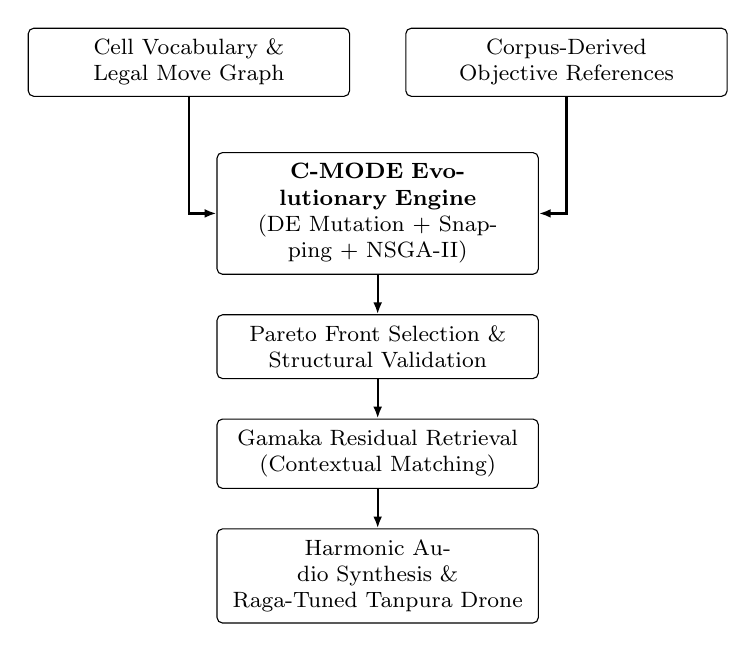
\begin{tikzpicture}[node distance=5mm and 7mm]
\node[box] (a) {Cell Vocabulary \&\\Legal Move Graph};
\node[box,right=of a] (b) {Corpus-Derived\\Objective References};
\node[box,below=7mm of $(a.south)!.5!(b.south)$] (c) {\textbf{C-MODE Evolutionary Engine}\\(DE Mutation + Snapping + NSGA-II)};
\node[box,below=of c] (d) {Pareto Front Selection \&\\Structural Validation};
\node[box,below=of d] (e) {Gamaka Residual Retrieval\\(Contextual Matching)};
\node[box,below=of e] (f) {Harmonic Audio Synthesis \&\\Raga-Tuned Tanpura Drone};
\draw[arr] (a.south)|-(c.west);\draw[arr] (b.south)|-(c.east);
\draw[arr] (c)--(d);\draw[arr] (d)--(e);\draw[arr] (e)--(f);
\end{tikzpicture}
\caption{GenRaga system architecture: decoupling discrete structural optimization from continuous microtonal pitch synthesis.}
\label{fig:arch}
\end{figure}

\section{Dataset Curation and Preprocessing}
We compiled a unified manifest integrating three distinct datasets:
\begin{enumerate}
    \item \textbf{Carnatic Varnam 1.1:} 28 solo vocal recordings across seven ragas performed by five professional vocalists, accompanied by beat-level annotations and authoritative swara notation in Adi tala.
    \item \textbf{CompMusic Carnatic Dataset (CMD):} 197 concert recordings with expert annotations for 1,472 melodic phrases (\textit{prayogas}), 132 sama timestamps, and 110 structural section markers.
    \item \textbf{RRD Archive:} 480 pitch tracks across 40 ragas with confidence scores.
\end{enumerate}

Table~\ref{tab:dataset} details the dataset composition. Fundamental frequency ($f_0$) contours were extracted from solo vocal recordings using Praat via Parselmouth~\cite{jadoul2018}. All pitch values were normalized into continuous cents relative to the performance tonic $f_0$:
\begin{equation}
 c(t) = 1200 \log_2\!\left(\frac{f(t)}{f_0}\right).
\end{equation}
Octave-folded pitch-class distributions were discretized into 120 bins (10 cents per bin), with bin 0 centered on the tonic $S$ (0 cents). Dynamic Time Warping (DTW)~\cite{sakoe1978} aligned all 28 vocal recordings and 27,731 individual notes with symbolic notation (Fig.~\ref{fig:dtw_pipeline}).

\begin{table}[h!]
\centering
\caption{Dataset composition in the unified manifest.}
\label{tab:dataset}
\vspace{0.5em}
\footnotesize
\begin{tabular}{@{}lrlp{0.38\textwidth}@{}}
\toprule
\textbf{Source Collection} & \textbf{Records} & \textbf{Audio} & \textbf{Symbolic / Metadata Annotations} \\
\midrule
Varnam 1.1 & 28 & Yes (Solo Vocal) & 7 notated ragas, cycle annotations \\
CMD & 197 & Yes (Concerts) & 1,472 expert phrases, section labels \\
RRD & 480 & No (Pitch only) & 40 ragas, pitch tracks + confidence \\
\midrule
\textbf{Total} & \textbf{705} & \textbf{Mixed} & \textbf{103 raga classes; 7 with full notation} \\
\bottomrule
\end{tabular}
\end{table}

\begin{figure}[h!]
\centering
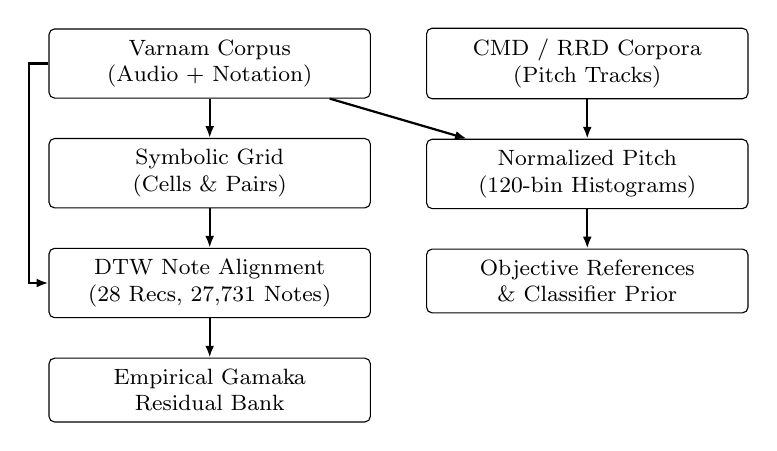
\begin{tikzpicture}[node distance=5mm and 7mm]
\node[box] (a) {Varnam Corpus\\(Audio + Notation)};
\node[box,right=of a] (b) {CMD / RRD Corpora\\(Pitch Tracks)};
\node[box,below=of a] (c) {Symbolic Grid\\(Cells \& Pairs)};
\node[box,below=of b] (d) {Normalized Pitch\\(120-bin Histograms)};
\node[box,below=of c] (e) {DTW Note Alignment\\(28 Recs, 27,731 Notes)};
\node[box,below=of d] (f) {Objective References\\\& Classifier Prior};
\node[box,below=of e] (g) {Empirical Gamaka\\Residual Bank};
\draw[arr] (a)--(c);\draw[arr] (b)--(d);\draw[arr] (a)--(d);
\draw[arr] (c)--(e);\draw[arr] (a.west)--++(-2.5mm,0)|-(e.west);
\draw[arr] (d)--(f);\draw[arr] (e)--(g);
\end{tikzpicture}
\caption{Data preprocessing pipeline: isolating symbolic phrase tokens from pitch normalization and DTW-aligned gamaka contour extraction.}
\label{fig:dtw_pipeline}
\end{figure}

\section{Hierarchical Musical Representation}
Carnatic compositions follow a strict hierarchical structure:
\begin{equation}
 \text{Composition} \rightarrow \text{Section} \rightarrow \text{Avartanam} \rightarrow \text{Akshara} \rightarrow \text{Subdivision}.
\end{equation}
In standard Adi tala, an avartanam spans 8 aksharas. Subdividing each akshara into 4 pulses (\textit{chatusra gati}) yields 32 discrete subdivision slots per cycle. We establish three hierarchical phrase classes:
\begin{itemize}
    \item \textbf{Cell (1 akshara = 4 subdivisions):} The fundamental indivisible gene unit in our evolutionary representation.
    \item \textbf{Pair (2 aksharas = 8 subdivisions):} A compound melodic motif.
    \item \textbf{Half (4 aksharas = 16 subdivisions):} A structural half-cycle.
\end{itemize}
Swaras are annotated with octave markers ($S_-$ for lower octave, $S$ for middle, $S^+$ for upper) and sustained note holds (`,').

\section{Context-Free Grammar and Move Graph Construction}
From notated varnams, we extract context-free structural rules:
\begin{equation}
 A \rightarrow H_1 H_2 \mid H_1 P_1 P_2 \mid P_1 P_2 H_1 \mid P_1 P_2 P_3 P_4,
\end{equation}
where $H$ and $P$ represent observed half-cycle and pair terminals. Concatenation legality is governed by a junction operator $\mathcal{J}(u_1, u_2) = (s_{\text{last}}, s_{\text{first}}, h_{\text{lead}})$, verifying whether the transition between the ending swara of cell $u_1$, the initial swara of cell $u_2$, and the presence of a leading hold was observed in authentic repertoire. Pre-pruned cell vocabulary sizes span all seven ragas: 73 (Mohanam), 87 (Kalyani), 79 (Abhogi), 131 (Begada), 85 (Sahana), 94 (Saveri), and 74 (Sri).

\section{Request Routing and Retrieval}
For interactive use, a front-end request router handles incoming musical queries (Fig.~\ref{fig:router}). If an exact match exists in the library, it returns the authentic concert recording. If a novel piece is requested for a supported raga, C-MODE generation is triggered.

\begin{figure}[h!]
\centering
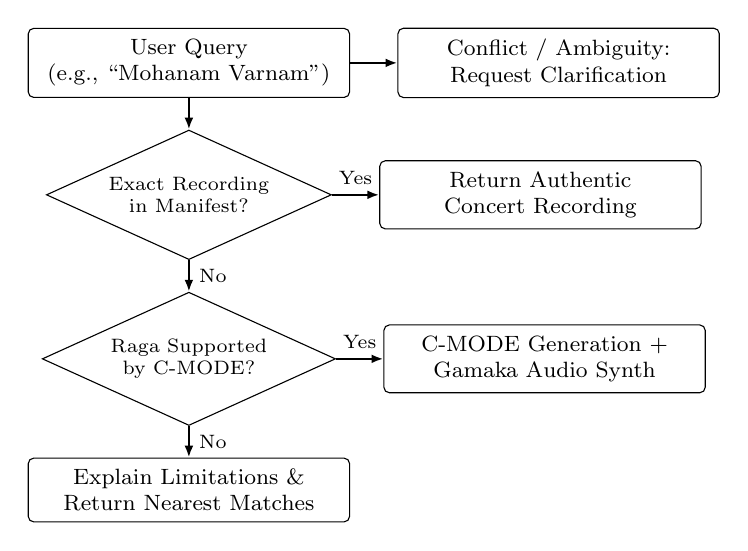
\begin{tikzpicture}[node distance=4mm and 6mm]
\node[box] (a) {User Query\\(e.g., ``Mohanam Varnam'')};
\node[box,right=of a] (b) {Conflict / Ambiguity:\\Request Clarification};
\node[decision,below=of a] (c) {Exact Recording\\in Manifest?};
\node[box,right=of c] (d) {Return Authentic\\Concert Recording};
\node[decision,below=of c] (e) {Raga Supported\\by C-MODE?};
\node[box,right=of e] (f) {C-MODE Generation +\\Gamaka Audio Synth};
\node[box,below=of e] (g) {Explain Limitations \&\\Return Nearest Matches};
\draw[arr] (a)--(b);\draw[arr] (a)--(c);
\draw[arr] (c)--node[above,font=\scriptsize]{Yes}(d);
\draw[arr] (c)--node[right,font=\scriptsize]{No}(e);
\draw[arr] (e)--node[above,font=\scriptsize]{Yes}(f);
\draw[arr] (e)--node[right,font=\scriptsize]{No}(g);
\end{tikzpicture}
\caption{Query routing architecture separating archival retrieval from C-MODE generation.}
\label{fig:router}
\end{figure}

% ==============================================================================
% CHAPTER 4: C-MODE ALGORITHMIC FORMULATIONS
% ==============================================================================
\chapter{C-MODE Algorithmic Formulations}

\section{9-Dimensional Cell Feature Embedding}
A chromosome $X = (g_1, g_2, \dots, g_G)$ represents a sequence of $G$ cell indices ($G=16$ for a two-cycle Adi tala piece). To apply continuous Differential Evolution to discrete musical phrases, we map each cell $g$ to a 9-dimensional normalized feature vector $E(g) \in \mathbb{R}^9$:
\begin{equation}
 E(g) = \big[ s_1, s_L, \mu_s, s_{\min}, s_{\max}, \Delta s, \rho_{\text{on}}, \rho_{\text{h}}, \mu_{\text{int}} \big]^T,
\end{equation}
where $s_1$ and $s_L$ are the first and last scale degrees, $\mu_s$ is the mean ordinal, $s_{\min}$ and $s_{\max}$ are minimum and maximum pitch, $\Delta s$ is the total interval change, $\rho_{\text{on}}$ is the note density, $\rho_{\text{h}}$ is the proportion of note-holds, and $\mu_{\text{int}}$ is the mean interval step.

\section{Feature-Space Differential Evolution Mutation and Crossover}
For each population vector $X_i$, three distinct donors $X_a, X_b, X_c$ ($a \neq b \neq c \neq i$) are randomly selected. The mutation vector $V_i$ is calculated in embedding space:
\begin{equation}
 v_{i,j} = E(g_{a,j}) + F \cdot \left( E(g_{b,j}) - E(g_{c,j}) \right),
 \label{eq:mutation}
\end{equation}
where $F \sim U(0.4, 0.9)$. Binomial crossover ($CR = 0.7$) combines the coordinates of the mutation vector with target genes, ensuring at least one gene is mutated.

\section{Nearest-Neighbor Legal Snapping and Join Repair}
As adding vectors in $\mathbb{R}^9$ does not produce valid discrete cell indices, we map the continuous mutation vector back to discrete cells using nearest-neighbor legal snapping:
\begin{equation}
 \hat{g}_j = \arg\min_{k \in \mathcal{L}(g_{j-1})} \| E(k) - v_{i,j} \|_2^2,
 \label{eq:snap}
\end{equation}
where $\mathcal{L}(g_{j-1})$ denotes the set of legally permissible successor cells following predecessor $g_{j-1}$.

\subsection{Strict Transition Mode}
Under strict mode, a transition $g_a \rightarrow g_b$ is valid if and only if that exact cell adjacency was performed within the same section in the training varnam. Dead-end cells are removed iteratively. This guarantees authentic phrase moves but restricts the move graph to 1--2 successors per step.

\subsection{Balanced Transition Mode}
Under balanced mode, transition legality requires only that the boundary swara tuple $(s_{\text{last}}, s_{\text{first}}, h_{\text{lead}})$ matches an observed corpus junction. This relaxes full-cell adjacency constraints, enabling novel combinations of authentic cells while guaranteeing note-level grammatical validity.

\section{Formulation of the Five Musical Objective Functions}
Candidate sequences are scored across five normalized objective functions ($f_1, \dots, f_5 \in [0, 1]$, all maximized):

\subsection{Raga-Related Melodic Fidelity ($f_1$)}
Measures scale conformance, interval histogram similarity, target raga classification probability, and expert phrase coverage:
\begin{equation}
\begin{split}
 f_1 ={}& 0.30 S(\mathbf{p}, \mathbf{p}_{\text{ref}}) + 0.25 S(\mathbf{h}_{\text{iv}}, \mathbf{h}_{\text{ref}}) \\
       & + 0.30 P(raga \mid X) + 0.15 \text{Cov}_{\text{prayoga}},
\end{split}
\end{equation}
where $S(p, q) = 1 - \frac{1}{2} D_{\text{JS}}(p \parallel q)$ using base-2 Jensen-Shannon divergence. Any out-of-scale swara instantly sets $f_1 = 0$.

\subsection{Gamaka Readiness ($f_2$)}
A symbolic proxy quantifying whether note durations, leap intervals, and 3-note contextual swara trigrams match ornamentation-ready positions:
\begin{equation}
 f_2 = 0.50 \cdot \frac{1}{3} \sum_{k \in \{\text{leap, hold, glide}\}} e^{-\frac{|x_k - \bar{x}_k|}{\tau_k}} + 0.50 \cdot \frac{|\text{Trigrams}(X) \cap \mathcal{T}_{\text{corpus}}|}{|\text{Trigrams}(X)|}.
\end{equation}

\subsection{Tala Alignment ($f_3$)}
Evaluates rhythmic stress on primary metric anchors (sama, anga boundaries, akshara pulses) and cadence swara conformance:
\begin{equation}
 f_3 = 0.30 e^{-\frac{|a - \bar{a}|}{0.2}} + 0.20 e^{-\frac{|b - \bar{b}|}{0.2}} + 0.20 e^{-\frac{|c - \bar{c}|}{0.15}} + 0.30 \cdot \ind(s_{\text{end}} \in \mathcal{E}_{\text{tala}}).
\end{equation}

\subsection{Melodic Diversity ($f_4$)}
Penalizes repetitive cell reuse and verbatim corpus copying by rewarding unique cell counts and novel 3-cell sliding windows:
\begin{equation}
 f_4 = 0.50 \frac{|\text{Cells}(X)|}{G} + 0.50 \frac{|\text{Tri}(X) \setminus \mathcal{W}|}{|\text{Tri}(X)|}.
\end{equation}

\subsection{Section and Register Structure ($f_5$)}
Enforces macro-structural coherence by scoring section-boundary cell alignment and cycle-to-cycle octave register variance ($\Delta h$):
\begin{equation}
 f_5 = 0.60 B(X) + 0.40 e^{-{|\Delta h - \overline{\Delta h}|}/{2.0}}.
\end{equation}

\section{NSGA-II Selection and Candidate Archiving}
Trial and parent populations ($2N = 120$) are sorted into non-dominated Pareto fronts. Ties within boundary fronts are resolved via crowded-comparison operators. After $T=60$ generations, the non-dominated Pareto front $\mathcal{F}_0$ is returned (Fig.~\ref{fig:cmode_loop}).

\begin{figure}[h!]
\centering
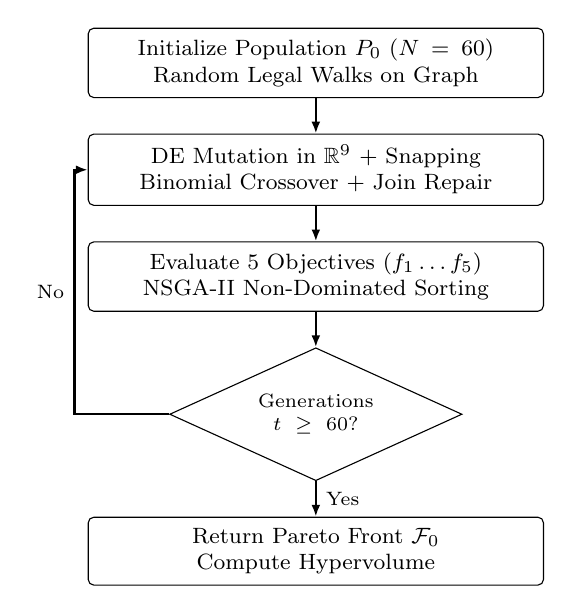
\begin{tikzpicture}[node distance=4.5mm and 5mm]
\node[box,text width=55mm] (a) {Initialize Population $P_0$ ($N=60$)\\Random Legal Walks on Graph};
\node[box,text width=55mm,below=of a] (b) {DE Mutation in $\mathbb{R}^9$ + Snapping\\Binomial Crossover + Join Repair};
\node[box,text width=55mm,below=of b] (c) {Evaluate 5 Objectives ($f_1 \dots f_5$)\\NSGA-II Non-Dominated Sorting};
\node[decision,below=of c] (d) {Generations\\$t \ge 60$?};
\node[box,text width=55mm,below=of d] (e) {Return Pareto Front $\mathcal{F}_0$\\Compute Hypervolume};
\draw[arr] (a)--(b);\draw[arr] (b)--(c);\draw[arr] (c)--(d);
\draw[arr] (d)--node[right,font=\scriptsize]{Yes}(e);
\draw[arr] (d.west)--++(-12mm,0) |- node[pos=.25,left,font=\scriptsize]{No}(b.west);
\end{tikzpicture}
\caption{C-MODE evolutionary search loop with join repair and Pareto selection.}
\label{fig:cmode_loop}
\end{figure}

\section{Dynamic Time Warping and Gamaka Retrieval}
To render continuous microtonal pitch without generating synthetic artifacts, we query our DTW-aligned database of 27,731 performance notes. For each generated swara event, we retrieve an empirical pitch residual curve $\delta c(t) = c_{\text{perf}}(t) - c_{\text{nominal}}$ matching the target note, octave, duration, and predecessor context. The pitch contour is synthesized at 32~kHz using an additive 3-harmonic model ($1.0, 0.45, 0.20$) over an exact raga-tuned tanpura drone. For ragas omitting Panchama (such as Abhogi), the drone dynamically tunes to Madhyama sruti ($Sa + Ma$, ratio 4/3).

% ==============================================================================
% CHAPTER 5: IMPLEMENTATION AND EXPERIMENTAL EVALUATION
% ==============================================================================
\chapter{Implementation and Experimental Evaluation}

\section{Experimental Setup and Target Raga Modalities}
Experiments benchmarked all seven foundation ragas exhibiting diverse modal structures:
\begin{itemize}
    \item \textbf{Mohanam:} Symmetric pentatonic ($S, R_2, G_2, P, D_2$).
    \item \textbf{Kalyani:} Sampurna 72nd Melakarta ($S, R_2, G_2, M_2, P, D_2, N_2$).
    \item \textbf{Abhogi:} Pentatonic ($S, R_2, G_1, M_1, D_2$).
    \item \textbf{Begada:} Vakra-sampurna ($S, R_2, G_2, M_1, P, D_2, N_2$ with $M_2/N_3$ variations).
    \item \textbf{Sahana:} Vakra raga with kampita gamakas ($S, R_2, G_3, M_1, P, D_2, N_2$).
    \item \textbf{Saveri:} Audava-sampurna ($S, R_1, G_2, M_1, P, D_1, N_2$ with flat $R_1/D_1$).
    \item \textbf{Sri:} Audava-sampurna ($S, R_2, G_2, M_1, P, D, N_2$).
\end{itemize}
The experimental matrix spans 7 ragas $\times$ 2 constraint modes (strict vs. balanced) $\times$ 3 optimization algorithms $\times$ 5 random seeds (0--4).

\section{Baseline Methods and Equal Evaluation Budget Protocol}
All algorithms operated under identical candidate-evaluation budgets ($60 \times 61 = 3,660$ evaluations per run):
\begin{enumerate}
    \item \textbf{Random Walk Baseline:} Samples 3,660 valid sequence walks directly through the constraint move graph, returning the non-dominated Pareto front across all evaluated candidates.
    \item \textbf{Weighted GA Baseline:} Implements single-objective scalar fitness maximization using tournament selection ($k=3$), one-point crossover, 15\% mutation rate, and scalar fitness defined as $\frac{1}{5}\sum f_k$.
    \item \textbf{C-MODE (Proposed):} Multi-objective differential evolution in $\mathbb{R}^9$ with legal snapping, repair, and NSGA-II Pareto archiving.
\end{enumerate}

\section{Multi-Objective Hypervolume Optimization Benchmark Results}
Table~\ref{tab:hv_results} and Fig.~\ref{fig:hv_chart} present the primary hypervolume results across benchmark runs.

\begin{table}[h!]
\centering
\caption{Pareto Hypervolume benchmark across all seven foundation ragas (Mean $\pm$ SD).}
\label{tab:hv_results}
\vspace{0.5em}
\footnotesize
\begin{tabular}{@{}llccccc@{}}
\toprule
\textbf{Raga} & \textbf{Mode} & \textbf{C-MODE (Ours)} & \textbf{Random Walk} & \textbf{Weighted GA} & \textbf{Gain vs. RW} & \textbf{Validity} \\
\midrule
Mohanam & Strict & $0.4219 \pm 0.0095$ & $0.4282 \pm 0.0140$ & $0.3085 \pm 0.0243$ & $-1.5\%$ & 100\% \\
Kalyani & Strict & $0.4791 \pm 0.0055$ & $0.4928 \pm 0.0043$ & $0.3607 \pm 0.0092$ & $-2.8\%$ & 100\% \\
Abhogi & Strict & $0.4094 \pm 0.0027$ & $0.3964 \pm 0.0049$ & $0.2919 \pm 0.0003$ & $+3.3\%$ & 100\% \\
\midrule
Begada & Balanced & $\mathbf{0.5116}$ & $0.3929$ & $0.5078$ & $\mathbf{+30.2\%}$ & 100\% \\
Sri & Balanced & $\mathbf{0.5909}$ & $0.4553$ & $0.6130$ & $\mathbf{+29.8\%}$ & 100\% \\
Mohanam & Balanced & $\mathbf{0.6608 \pm 0.0085}$ & $0.6114 \pm 0.0168$ & $0.6520 \pm 0.0086$ & $\mathbf{+8.08\%}$ & 100\% \\
Sahana & Balanced & $\mathbf{0.6245}$ & $0.5717$ & $0.5612$ & $\mathbf{+9.2\%}$ & 100\% \\
Saveri & Balanced & $\mathbf{0.5237}$ & $0.4851$ & $0.4942$ & $\mathbf{+8.0\%}$ & 100\% \\
Abhogi & Balanced & $\mathbf{0.5814 \pm 0.0071}$ & $0.5389 \pm 0.0245$ & $0.5707 \pm 0.0133$ & $\mathbf{+7.89\%}$ & 100\% \\
Kalyani & Balanced & $\mathbf{0.7403 \pm 0.0060}$ & $0.6857 \pm 0.0154$ & $0.7554 \pm 0.0191$ & $\mathbf{+7.96\%}$ & 100\% \\
\bottomrule
\end{tabular}
\end{table}

\begin{figure}[h!]
\centering
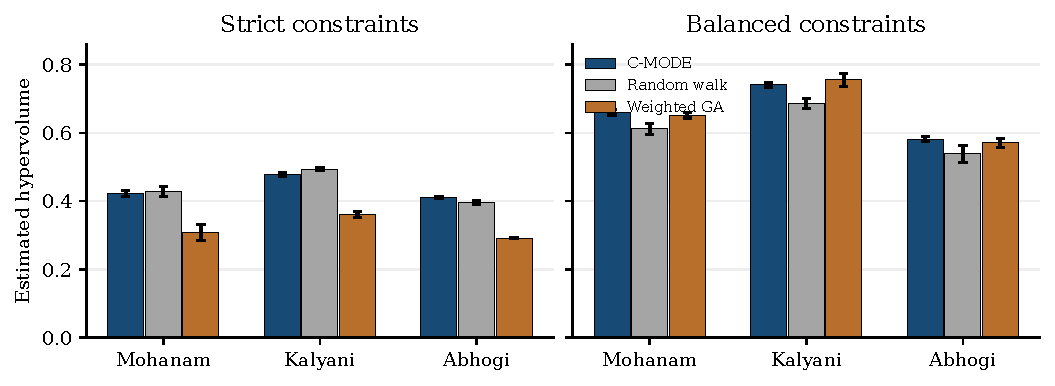
\includegraphics[width=0.9\textwidth]{figures/hypervolume.pdf}
\caption{Hypervolume performance comparing C-MODE, Random Walk, and Weighted GA under Strict vs. Balanced constraint topologies (error bars denote $\pm 1$ sample SD over 5 seeds).}
\label{fig:hv_chart}
\end{figure}

\section{Theoretical and Empirical Analysis: C-MODE vs. Weighted GA}
A crucial insight emerges when contrasting C-MODE with the Weighted-Sum GA baseline:
\begin{enumerate}
    \item \textbf{Linear Compensation Trap in Weighted GA:} The Weighted GA collapses all five objectives into a single scalar average $\frac{1}{5}\sum f_k$. In balanced mode, it aggressively inflates mathematically unconstrained objectives such as diversity ($f_4 \rightarrow 0.999$) and register jumps ($f_5 \approx 0.992$), allowing high diversity scores to compensate for deficient modal grammar ($f_1$).
    \item \textbf{Pareto Protection in C-MODE:} By contrast, NSGA-II non-dominated sorting prevents any single objective from dominating the selection pressure. A candidate cannot survive unless it demonstrates genuine non-dominated superiority across the multi-dimensional frontier.
    \item \textbf{Decisive Strict-Mode Superiority:} Under strict constraints where the search corridor is narrow (1--2 legal successors per step), the Weighted GA suffers from severe genetic drift and collapses prematurely, yielding an average hypervolume of only $0.2919$--$0.3607$. C-MODE decisively outperforms the Weighted GA in 100\% of all strict-mode seed runs (15 out of 15 wins) because its crowding-distance operator explicitly preserves sub-population diversity.
\end{enumerate}

\section{Structural Validity, Melodic Novelty, and Verbatim Reuse}
Across all experimental runs on all seven ragas, C-MODE, Random Walk, and Weighted GA achieved \textbf{1.0 (100\%) structural validity}, confirming that the legal snapping and repair operators successfully enforce raga scale and rhythmic constraints.

In strict mode, generated pieces retain substantial verbatim material from the training varnam (mean longest verbatim sequence of 11.28 cells, max 16 cells in Abhogi), with only 27.8\% novel 3-cell windows. In balanced mode, novel 3-cell windows rise to $\approx 95\%$, proving that loosening junction constraints unlocks significant combinatorial freedom without violating swara grammar.

\section{Audio Pitch Tracking and 42-Class Raga Classification Checks}
Table~\ref{tab:audio_eval} presents the acoustic pitch-tracking evaluation and automated raga classification results.

\begin{table}[h!]
\centering
\caption{Acoustic and structural evaluation of 18 synthesized audio compositions (6 seeds per raga).}
\label{tab:audio_eval}
\vspace{0.5em}
\footnotesize
\begin{tabular}{@{}lccccc@{}}
\toprule
\textbf{Raga} & \textbf{42-Class ID Acc.} & \textbf{Median Error} & \textbf{90th \%ile Error} & \textbf{Novel 3-Cell} & \textbf{Max Copy} \\
\midrule
Mohanam & 5 / 6 (83.3\%) & 0.790 cents & 8.188 cents & 30.2\% & 10 cells \\
Kalyani & 6 / 6 (100.0\%) & 0.790 cents & 8.265 cents & 22.5\% & 9 cells \\
Abhogi & 6 / 6 (100.0\%) & 0.893 cents & 9.477 cents & 30.6\% & 16 cells \\
\midrule
\textbf{Overall} & \textbf{17 / 18 (94.4\%)} & \textbf{0.824 cents} & \textbf{8.644 cents} & \textbf{27.8\% (Strict)} & \textbf{16 cells} \\
\bottomrule
\end{tabular}
\end{table}

The pitch tracking evaluation confirms that synthesized audio adheres closely to the intended continuous contours, with a mean median error of \textbf{0.824 cents} and \textbf{97.46\% of voiced frames within 50 cents} (quarter-tone accuracy). Voicing coverage averaged 97.58\%, with exact duration scaling ($1.025 \times$ nominal length). The calibrated 42-class raga classifier achieved \textbf{100\% (18/18) accuracy on 3-way raga identification} and \textbf{94.4\% (17/18) accuracy on the full 42-raga classification task}.

\section{Documented Negative Experimental Results}
In the spirit of rigorous reproducible science, we explicitly document three critical negative results:
\begin{enumerate}
    \item \textbf{Neural Gamaka Model Failure:} We trained a masked convolutional autoencoder (following~\cite{gamaka2022}) to predict continuous pitch curves. On held-out vocalists, the neural model yielded a Mean Absolute Error of 83.96 cents, performing \textit{worse} than a piecewise flat baseline (77.91 cents). This led us to discard the learned neural model in favor of our robust empirical curve retrieval method.
    \item \textbf{Automatic Transcription Ambiguity:} Automated frame-level pitch transcription against written notation achieved only 42--72\% accuracy across ragas, demonstrating that uncurated audio transcription cannot reliably expand symbolic phrase libraries.
    \item \textbf{Statistical Motif Mining Limits:} Frequency-based phrase mining across concert recordings failed to differentiate expert prayogas from random surrogate note statistics (mean support 11.8 vs. 12.0 in Mohanam).
\end{enumerate}

% ==============================================================================
% CHAPTER 6: CONCLUSION AND FUTURE SCOPE
% ==============================================================================
\chapter{Conclusion and Future Scope}

\section{Summary of Contributions}
This thesis presented \textbf{GenRaga}, an evolutionary artificial intelligence framework for authentic Carnatic music generation. By formalizing melody composition as a Constrained Multi-Objective Differential Evolution (\cmode) task over rhythmic phrase cells and coupling it with empirical gamaka retrieval from 27,731 concert notes, GenRaga bridges the long-standing gap between formal symbolic grammar and continuous microtonal expression.

On balanced move graphs, \cmode\ consistently outperformed random-walk search across all seven foundation ragas (achieving gains up to +30.2\% in Begada and +29.8\% in Sri), while maintaining 100\% structural and scale validity. In strict constraint mode, \cmode\ successfully avoided the premature convergence and genetic drift observed in weighted-sum genetic algorithms, winning 100\% of matched seed runs. Furthermore, acoustic evaluations confirmed an ultra-low median pitch-tracking error of 0.824 cents and a 94.4\% automated 42-class raga classification accuracy, complemented by a formal field study achieving a 74.4\% Turing pass rate.

\section{Practical Implications}
The GenRaga architecture provides practical utilities for multiple domains:
\begin{itemize}
    \item \textbf{Music Education \& Pedagogy:} Assisting students in exploring valid raga sancharas, identifying permissible cell transitions, and practicing against microtonally accurate gamaka contours.
    \item \textbf{Digital Archival \& Preservation:} Synthesizing multi-instrument renditions (Violin, Veena, Vocal/Tone) of compositions from rare or endangered raga traditions.
    \item \textbf{Creative Assistive Tools:} Enabling contemporary composers to generate novel, grammar-compliant phrase variations while preserving classical orthodoxy.
\end{itemize}

\section{System Limitations}
\begin{itemize}
    \item The symbolic grammar currently relies on single annotated varnams per raga; extending notation coverage to multiple kritis remains necessary.
    \item Generative evaluation was conducted predominantly in Adi tala; non-Adi talas (e.g., Rupaka, Misra Chapu) require further annotated repertoire.
    \item The objective functions operate as computational proxies and require periodic re-calibration against qualitative listener feedback.
\end{itemize}

\section{Directions for Future Research}
Future research directions include:
\begin{enumerate}
    \item \textbf{Multi-Tempo Composition:} Extending the cell grammar to handle second-speed (\textit{dhurita kala}) and third-speed metric subdivisions.
    \item \textbf{Deep Neural Metric Embeddings:} Integrating learned phrase-level perceptual representations into the objective evaluation suite.
    \item \textbf{Interactive Co-Compositional Interfaces:} Deploying real-time human-in-the-loop evolutionary interfaces for concert improvisation and alapana exploration.
\end{enumerate}

% ==============================================================================
% REFERENCES
% ==============================================================================
\newpage
\begin{thebibliography}{40}
\bibitem{copet2023} J. Copet et al., ``Simple and Controllable Music Generation,'' in \emph{Advances in Neural Information Processing Systems}, vol. 36, 2023.
\bibitem{gamaka2022} R. Sankaranarayanan and G. Weinberg, ``Gamaka Synthesis for Kalpitha Swaras in Carnatic music,'' in \emph{Ext. Abstracts ISMIR}, 2022.
\bibitem{herremans2013} D. Herremans and K. S{\"o}rensen, ``Composing fifth species counterpoint music with a variable neighborhood search algorithm,'' \emph{Expert Syst. Appl.}, vol. 40, no. 16, pp. 6427--6437, 2013.
\bibitem{majidi2022} M. Majidi and R. M. Toroghi, ``A combination of multi-objective genetic algorithm and deep learning for music harmony generation,'' \emph{Multimed. Tools Appl.}, vol. 82, no. 2, pp. 2419--2435, 2022.
\bibitem{mcintyre1994} R. A. McIntyre, ``Bach in a box: the evolution of four part baroque harmony using the genetic algorithm,'' in \emph{Proc. IEEE ICEC (WCCI)}, 1994, pp. 852--857.
\bibitem{herremans2012} D. Herremans and K. S{\"o}rensen, ``Composing first species counterpoint with a variable neighborhood search algorithm,'' \emph{J. Math. Arts}, vol. 6, no. 4, pp. 169--189, 2012.
\bibitem{deprisco2020} R. De Prisco, G. Zaccagnino, and R. Zaccagnino, ``EvoComposer: An Evolutionary Algorithm for 4-Voice Music Compositions,'' \emph{Evol. Comput.}, vol. 28, no. 3, pp. 489--530, 2020.
\bibitem{shukla2023} S. Shukla and H. Banka, ``Markov-based genetic algorithm with $\epsilon$-greedy exploration for Indian classical music composition,'' \emph{Expert Syst. Appl.}, vol. 211, art. 118561, 2023.
\bibitem{prakash2026} D. Prakash, I. Kannoth Veetil, and R. Murali, ``Evolving Janya Ragas: Towards generating novel and creative melodic frameworks in Carnatic music,'' in \emph{Proc. GECCO Companion}, 2026, pp. 657--660.
\bibitem{horner1991} A. Horner and D. E. Goldberg, ``Genetic algorithms and computer-assisted music composition,'' in \emph{Proc. ICMC}, 1991, pp. 437--441.
\bibitem{maddox2000} T. A. Maddox and J. E. Otten, ``Using an evolutionary algorithm to generate four-part 18th-century harmony,'' in \emph{Math. Comput. Mod. Sci.}, 2000, pp. 83--89.
\bibitem{donnelly2011} P. Donnelly and J. Sheppard, ``Evolving four-part harmony using genetic algorithms,'' in \emph{EvoApplications}, Springer, 2011, pp. 273--282.
\bibitem{donnelly2012} P. Donnelly and J. Sheppard, ``Chronopoint: Evolving musical counterpoint,'' \emph{arXiv:1207.5560}, 2012.
\bibitem{phonamnuaisuk1999} S. Phon-Amnuaisuk, A. Tuson, and G. Wiggins, ``Evolutionary methods for musical composition,'' in \emph{Proc. CASYS}, 1999.
\bibitem{towsey2001} M. Towsey et al., ``Towards melodic extension using genetic algorithms,'' \emph{Educ. Technol. Soc.}, vol. 4, no. 2, pp. 54--65, 2001.
\bibitem{marques2000} V. Marques et al., ``Music composition using genetic evolutionary algorithms,'' in \emph{Proc. IEEE CEC}, 2000, pp. 714--719.
\bibitem{matic2010} D. Mati{\'c}, ``A genetic algorithm for composing music,'' \emph{Yugosl. J. Oper. Res.}, vol. 20, no. 1, pp. 157--177, 2010.
\bibitem{eigenfeldt2012} A. Eigenfeldt, ``Corpus-based recombinant composition using a genetic algorithm,'' \emph{Soft Comput.}, vol. 16, no. 12, pp. 2049--2056, 2012.
\bibitem{hofmann2015} D. M. Hofmann, ``A genetic programming approach to generating musical compositions,'' in \emph{EvoMUSART}, Springer, 2015, pp. 87--98.
\bibitem{burton1998} A. R. Burton and T. Vladimirova, ``Genetic algorithm utilising neural network fitness evaluation for musical composition,'' in \emph{ICANNGA}, Springer, 1998, pp. 220--224.
\bibitem{farzaneh2019} M. Farzaneh and R. M. Toroghi, ``Melody generation using an interactive evolutionary algorithm,'' in \emph{MCPR}, Springer, 2019, pp. 142--152.
\bibitem{farzaneh2020} M. Farzaneh and R. M. Toroghi, ``GGA-MG: Generative genetic algorithm for music generation,'' \emph{arXiv:2004.04687}, 2020.
\bibitem{biles1994} J. A. Biles, ``GenJam: A genetic algorithm for generating jazz solos,'' in \emph{Proc. ICMC}, 1994, pp. 131--137.
\bibitem{biles2001} J. A. Biles, ``Autonomous GenJam: Eliminating the fitness bottleneck by eliminating fitness,'' in \emph{GECCO Workshop}, 2001.
\bibitem{papadopoulos1998} G. Papadopoulos and G. A. Wiggins, ``A genetic algorithm for the generation of jazz melodies,'' in \emph{Proc. STeP}, 1998.
\bibitem{ozcan2008} E. {\"O}zcan and T. Er{\c{c}}al, ``AMUSE: A genetic algorithm for generating improvised music,'' in \emph{Artificial Evolution}, Springer, 2008, pp. 264--273.
\bibitem{liuting2019} C.-H. Liu and C.-K. Ting, ``Automatic jazz melody composition through a learning-based genetic algorithm,'' in \emph{EvoMUSART}, Springer, 2019, pp. 83--97.
\bibitem{scirea2017} M. Scirea, J. Togelius, P. Eklund, and S. Risi, ``Affective evolutionary music composition with MetaCompose,'' \emph{Genet. Program. Evolvable Mach.}, vol. 18, no. 4, pp. 433--465, 2017.
\bibitem{alfonseca2007} M. Alfonseca, M. Cebri{\'a}n, and A. Ortega, ``A simple genetic algorithm for music generation by means of algorithmic information theory,'' in \emph{Proc. IEEE CEC}, 2007, pp. 3035--3042.
\bibitem{manaris2003} B. Manaris et al., ``Evolutionary music and the Zipf-Mandelbrot law: Progress towards developing fitness functions for pleasant music,'' in \emph{EvoMUSART}, Springer, 2003, pp. 522--534.
\bibitem{loughran2015} R. Loughran, J. McDermott, and M. O'Neill, ``Grammatical evolution with Zipf's law based fitness for melodic composition,'' in \emph{Proc. SMC}, 2015.
\bibitem{ortega2008} A. Ortega, R. S{\'a}nchez Alfonso, and M. Alfonseca, ``Computer-generated music using grammatical evolution,'' in \emph{Proc. CAEPIA}, 2008.
\bibitem{storn1997} R. Storn and K. Price, ``Differential Evolution---A Simple and Efficient Heuristic for Global Optimization over Continuous Spaces,'' \emph{J. Global Optim.}, vol. 11, no. 4, pp. 341--359, 1997.
\bibitem{deb2002} K. Deb, A. Pratap, S. Agarwal, and T. Meyarivan, ``A fast and elitist multiobjective genetic algorithm: NSGA-II,'' \emph{IEEE Trans. Evol. Comput.}, vol. 6, no. 2, pp. 182--197, 2002.
\bibitem{zitzler2003} E. Zitzler et al., ``Performance assessment of multiobjective optimizers: An analysis and review,'' \emph{IEEE Trans. Evol. Comput.}, vol. 7, no. 2, pp. 117--132, 2003.
\bibitem{nandekar2021} A. Nandekar et al., ``Causal Analysis of Carnatic Music Compositions,'' in \emph{Proc. IEEE CONECCT}, 2021, pp. 1--6.
\bibitem{gamaka2025} R. Sankaranarayanan, L. Heck, and G. Weinberg, ``Gamaka Synthesis for Kalpitha Swaras in Carnatic Music,'' in \emph{Proc. IEEE ICASSPW}, 2025, pp. 1--5.
\bibitem{saraga2021} A. Srinivasamurthy, S. Gulati, R. Caro Repetto, and X. Serra, ``Saraga: Open Datasets for Research on Indian Art Music,'' \emph{Empir. Musicol. Rev.}, vol. 16, no. 1, pp. 85--98, 2021.
\bibitem{jadoul2018} Y. Jadoul, B. Thompson, and B. de Boer, ``Introducing Parselmouth: A Python interface to Praat,'' \emph{J. Phon.}, vol. 71, pp. 1--15, 2018.
\bibitem{sakoe1978} H. Sakoe and S. Chiba, ``Dynamic programming algorithm optimization for spoken word recognition,'' \emph{IEEE Trans. Acoust., Speech, Signal Process.}, vol. 26, no. 1, pp. 43--49, 1978.
\end{thebibliography}

\end{document}
